\documentclass[cs4size,a4paper]{ctexart}   

\usepackage{cite}
\usepackage{url}
%===数学符号公式===
\usepackage{amsmath}    					% AMS LaTeX宏包
\usepackage[style=1]{mdframed}
\usepackage{amsthm}
\usepackage{amssymb}
\usepackage{bm}                      	% 数学公式中的黑斜体
\usepackage{bbm}
\usepackage{amsfonts}
\usepackage{mathrsfs}                	% 英文花体字 体
\usepackage{bbding,manfnt}    			% 一些图标,如 \dbend
\usepackage{lettrine}                	% 首字下沉,命令\lettrine
\def\attention{\lettrine[lines=2,lraise=0,nindent=0em]{\large\textdbend\hspace{1mm}}{}}
\usepackage{longtable}
\usepackage{enumerate}
\usepackage[toc,page]{appendix}
\usepackage{geometry}         			% 页边距调整
\geometry{top=3.0cm,bottom=2.7cm,left=2.5cm,right=2.5cm}
\usepackage[colorinlistoftodos,prependcaption,textsize=small]{todonotes}
%===公式按章编号===
\numberwithin{equation}{section}
\numberwithin{table}{section}
\numberwithin{figure}{section}
%===基本格式预置===
\usepackage{fancyhdr}
\pagestyle{fancy}
\fancyhf{}  
\fancyhead[C]{\zihao{5}  \kaishu 大创文献综述}
\fancyfoot[C]{~\zihao{5} \thepage~}
\renewcommand{\headrulewidth}{0.75pt} 
\CTEXsetup[format={\centering\bfseries\zihao{-2}},name={第, 章}]{section}
\CTEXsetup[nameformat={\bfseries\zihao{3}}]{subsection}
\CTEXsetup[nameformat={\bfseries\zihao{4}}]{subsubsection}
%===图形支持宏包===
\usepackage{graphicx}        			% 嵌入png图像
\usepackage{subfigure}
\usepackage{float}
\graphicspath{{figure/}}
\usepackage{color,xcolor}     			% 支持彩色文本、底色、文本框等
\usepackage[colorlinks,linkcolor=blue,anchorcolor=blue,citecolor=blue]{hyperref}
%\usepackage{caption}
\usepackage[ruled,linesnumbered]{algorithm2e}
%\captionsetup{figurewithin=section}
%===源码和流程图===
\usepackage{listings,fontspec}         	% 粘贴源代码
\newfontfamily\consolas{Consolas}
\definecolor{mygreen}{rgb}{0,0.6,0}
\definecolor{mygray}{rgb}{0.5,0.5,0.5}
\definecolor{mymauve}{rgb}{0.58,0,0.82}
%===颜色===
\usepackage{color,xcolor}
\definecolor{dkgreen}{rgb}{0,0.6,0}
\definecolor{gray}{rgb}{0.5,0.5,0.5}
\definecolor{mauve}{rgb}{0.58,0,0.82}
\usepackage{xcolor}
\lstset{ %
%numberstyle=\tiny\monaco,
%numberstyle=\color[RGB]{0,192,192},
%backgroundcolor=\color{white},   		% choose the background color
backgroundcolor=\color[RGB]{245,245,244},
%backgroundcolor=\color[rgb]{1,1,0.76},
basicstyle=\footnotesize\consolas,       % size of fonts used for the code
identifierstyle=\footnotesize\consolas, 
columns=fullflexible,
breaklines=true,                 		% automatic line breaking only at whitespace
captionpos=b,                    		% sets the caption-position to bottom
tabsize=2,
commentstyle=\color{mygreen}\consolas,   % comment style
%commentstyle=\it\color[RGB]{0,96,96},
escapeinside={\%*}{*)},          		% if you want to add LaTeX within your code
keywordstyle=\color{blue}\consolas,      % keyword style
stringstyle=\color{mymauve}\consolas,    % string literal style
%stringstyle=\rmfamily\slshape\color[RGB]{128,0,0},
frame=single,
rulesepcolor=\color{red!20!green!20!blue!20},
%identifierstyle=\color{red},
language=c++,
framexleftmargin=1.9mm,
xleftmargin=0.4em,
frame=none,
showstringspaces=false,
numbers=none,
}

%--------------------
\hypersetup{hidelinks}
\usepackage{booktabs}  
\usepackage{shorttoc}
\usepackage{tabu,tikz}
\usepackage{float}
\usepackage{multirow}

\tabcolsep=1ex
\tabulinesep=\tabcolsep
\newlength\tikzboxwidth
\newlength\tikzboxheight
\newcommand\tikzbox[1]{%
        \settowidth\tikzboxwidth{#1}%
        \settoheight\tikzboxheight{#1}%
        \begin{tikzpicture}
        \path[use as bounding box]
                (-0.5\tikzboxwidth,-0.5\tikzboxheight)rectangle
                (0.5\tikzboxwidth,0.5\tikzboxheight);
        \node[inner sep=\tabcolsep+0.5\arrayrulewidth,line width=0.5mm,draw=black]
                at(0,0){#1};
        \end{tikzpicture}%
        }
\makeatletter
\def\hlinew#1{%
  \noalign{\ifnum0=`}\fi\hrule \@height #1 \futurelet
   \reserved@a\@xhline}
   
\usepackage{CJK}
\usepackage{ifthen}
\newcommand{\HRule}{\rule{\linewidth}{0.5mm}}
\newcommand{\tabincell}[2]{\begin{tabular}{@{}#1@{}}#2\end{tabular}}%
%===使得公式随章节自动编号===
\makeatletter
\@addtoreset{equation}{section}
\makeatother
\renewcommand{\theequation}{\arabic{section}.\arabic{equation}}
%-------------------------
\usepackage{pythonhighlight}
\usepackage{tikz}                    
\usepackage{tikz-3dplot}
\usetikzlibrary{shapes,arrows,positioning}
%===正文开始===
\begin{document}
%===定理类环境定义===
\newtheorem{example}{例}              	% 整体编号
\newtheorem{algorithem}{算法}	
\newtheorem{theorem}{定理}            	% 按section编号
\newtheorem{definition}{定义}
\newtheorem{axiom}{公理}
\newtheorem{property}{性质}
\newtheorem{proposition}{命题}
\newtheorem{lemma}{引理}
\newtheorem{corollary}{推论}
\newtheorem{remark}{注解}
\newtheorem{condition}{条件}
\newtheorem{conclusion}{结论}
\newtheorem{assumption}{假设}
%===重定义===
\renewcommand{\contentsname}{目录}     
\renewcommand{\abstractname}{摘要} 
\renewcommand{\refname}{参考文献}     
\renewcommand{\indexname}{索引}
\renewcommand{\figurename}{图}
\renewcommand{\tablename}{表}
\renewcommand{\appendixname}{附录}
\renewcommand{\proofname}{证明}
%\renewcommand{\algorithm}{算法} 
\renewcommand\emph[1]{\textcolor{black}{\textbf{#1}}}
%===封皮和前言===
\begin{titlepage}
\begin{center}
% Upper part of the page

\includegraphics[width=0.30\textwidth]{logo}\\[1cm]    
\textsc{\Large Beijing University of Chemical Technology}\\[1.0cm]
\textsc{\Large Computing Methods}\\[0.5cm]
% Title
\HRule \\[0.8cm]
{\huge \bfseries 大创文献综述}\\[0.4cm]
\HRule \\[0.7cm]
% Author
\textsc{刘本佳,庄梓博,贺怀宇,李昊,王昕凯\\(排名不分先后)}
\tableofcontents 
\vfill
% Bottom of the page
{创建日期:2020年3月25日}\\
{更新日期:\today}
\end{center}
\end{titlepage}
\pagestyle{plain}
\pagenumbering{Roman}
\thispagestyle{empty}
%===正文===
\pagestyle{fancy}
\pagenumbering{arabic}

\abstract
不需要对整个场地进行定制(地面标识,摩擦系数),使其拥有特别高的快速部署和适应能力(对场地进行建模即可投入运行)
%===第一章===
\section{AGV研究进展}
AGV系统是集光、机、电、计算机于一体的高新技术。为了能够适应不同的使用要求和缩短新产品的开发周期,AGV的设计研究趋向于模块化,将AGV的各功能模块设计成不同的系列,再根据具体的使用要求进行组合。由于使用方便、费用低,分析验证AGV工程可行性时,现基本使用系统仿真方法。
仿真系统一般包括彩色图形输入与显示系统、仿真处理机和仿真语言。越来越多的AGV系统控制结构具有跟踪物料和储存信息的功能,以便允许与AGV间或任何其他控制器进行通信。设计AGV时的控制系统中的三个主要技术:AGV的导航(Navigation),AGV的路径规划(Layout designing),AGV的导引控制(Guidance)。
\subsection{AGV的导航(Navigation)}
导航技术是AGV技术的研究核心,其主要解决车辆位置获取、环境模型构建以及行驶路径规划等问题。国内外主流AGV导航方式分为固定路径导航和柔性路径导航两类。固定路径导航技术相对成熟,是国内AGV采用的主流导航方法,但该类技术无法满足运行路径需经常调整的情况。柔性路径导航技术应用较多的是激光引导、惯性导航、基于WIFI等无线信号定位的导引技术及视觉导航技术等。
视觉导航技术在上述两种形式导航技术中应用广泛。D.L.Boley等利用卡尔曼滤波器进行最优估计,有效降低噪声和提高实时性,利用车载摄像机和辅助传感器通过识别路标进行导航。美国卡内基·梅隆大学(CMU)研制的NAVLAB利用了神经网络技术,提高了其智能化程度。Horswill I采用单目视觉提取地面纹理,实现了车体在固定环境下的视觉导航。美国Kiva公司的Kiva系统控制AGV通过视觉识别贴在地面上的二维码信息,实现路径规划与导航。国内闵华松等提出了一种将IMU和体感摄像机相结合的地图构建算法,提高了导航地图的精度。李华等研制的THMR-V型AGV通过机器视觉算法检测车体与行车道的相对位置与方向信息,结合多种传感器融合检测实现在结构化道路环境中自主行驶。

\subsection{AGV的导引控制(Guidance)}
电磁感应导引已广泛应用;激光导引是目前采用的主流技术;视觉导引是研究的热点;惯性导引、超声波导引和磁石导引正被关注;标记追踪导向及图像传感器导向方式也同样值得重视。单导引技术不能解决成本、可靠性、灵活性和定位精度等性能指标之间的矛盾。AGV正向多导向方式、智能化发展,多种导向方式充分体现了无人搬运系统高效率、高柔性、高可靠性、低成本的发展特点。

\subsection{AGV的路径规划(Layout designing)}
现阶段的路径规划技术有两阶段控制策略、Petri网、遗传算法、TabuSearch算法(禁忌搜索算法)等方法。这些策略虽减少了在线运算的负担,但是随着节点数的增多,动态规划的负担加重,不适用于大规模的多AGV系统。而时间窗(Time-window)技术被应时提出,它有效地共享系统路径,解决了多AGV最优路径问题。
国内泰应鹏等利用A*算法启发式地为多个AGV进行规划路径,通过对时间窗(Time-window)的排布和更新解决了多AGV在路径规划中的碰撞冲突问题,通过动态地为多AGV分配优先级,提升了系统效率。方庆琯等提出以静态环境地图作为基础,结合新的免疫网络算法构成的一种实用的全局路径规划方法。S. Khanmohammadi等使用提出的基于混合模糊的方法,使AGV能朝着经过不同形状和位置的障碍物的目的地移动,并为AGV分配路径查找功能,可以降低中央控制器的计算复杂度,通过考虑机器人中的足够内存来解决局部规划问题。Minah Seo等采用Dijkstra算法在动态条件下实现了AGV的最佳路径规划,所提出的方法证明了AGV的能耗最小化,并以最佳路径改善了运行时间。

%===第二章===
\section{工程分解:硬件部分}

\subsection{AGV底盘}

\subsection{LiDAR传感器}

\subsection{RGBD传感器}

%===第三章===
\section{工程分解:软件部分}
\subsection{SLAM算法描述}
\subsubsection{SLAM定义}
同步定位与地图构建(SLAM或Simultaneous localization and mapping)是一种概念:希望机器人从未知环境的未知地点出发,在运动过程中通过重复观测到的地图特征(比如,墙角,柱子等)定位自身位置和姿态,再根据自身位置增量式的构建地图,从而达到同时定位和地图构建的目的。

在误差和噪音条件下,定位和地图构建技术上的复杂度不支持两者同时获得连续的解。即时定位与地图构建(SLAM)是这样一个概念:把两方面的进程都捆绑在一个循环之中,以此支持双方在各自进程中都求得连续解;不同进程中相互迭代的反馈对双方的连续解有改进作用。

同步定位与地图构建(SLAM)被定义为以下问题:在建立新地图模型或者改进已知地图的同时,在该地图模型上定位机器人。实际上,这两个核心问题如果分开解决,将毫无意义;必须同时求解。
即通过控制数据$u_{1:t}$和观测数据$z_{1:t}$来求解位姿和地图的联合概率分布
\begin{align}
    p\left(x_{1: t}, m | z_{1: t}, u_{1: t-1}\right)
\end{align}
\subsubsection{激光雷达:GMAPPING}
该算法\cite{1570477}是基于滤波SLAM框架的常用开源SLAM算法。基于RBpf粒子滤波算法,即将定位和建图过程分离,先进行定位再进行建图,即有以下表达式:
\begin{align}
    p\left(x_{1: t}, m | z_{1: t},\right.&\left.u_{1: t-1}\right) =p\left(m | x_{1: t}, z_{1: t}\right) \cdot p\left(x_{1: t} | z_{1: t}, u_{1: t-1}\right)
\end{align}
同时,GMAPPING在RBpf算法上做了两个主要改进:\textbf{改进提议分布}和\textbf{选择性重采样}。

改进的提议分布不但考虑运动(里程计)信息还考虑最近的一次观测(激光)信息这样就可以使提议分布的更加精确从而更加接近目标分布。选择性重采样通过设定阈值,只有在粒子权重变化超过阈值时才执行重采样从而大大减少重采样的次数。

\begin{figure}[H]
  \centering
  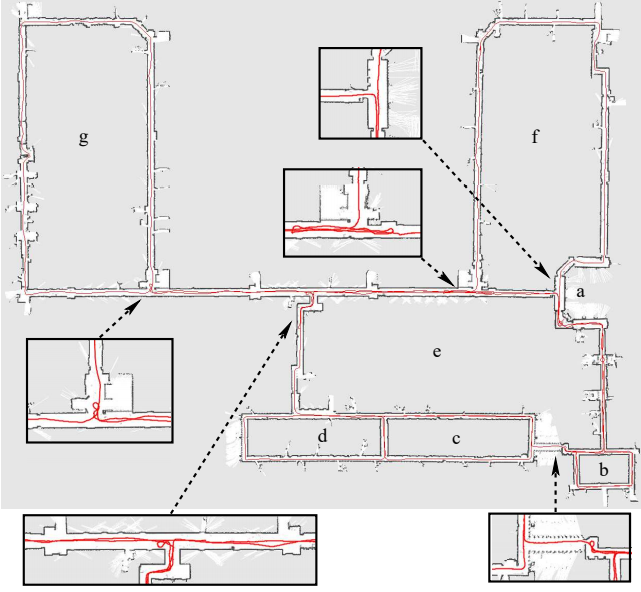
\includegraphics[width=0.6\textwidth]{figure/gmapping-1.png}
  \caption{机器人从标记为a的点开始,然后遍历标记为b的第一个循环。 然后,它在标记为c,d的循环中移动,并移回到标记为a的位置和标记为b的循环中。 它访问标记为f和g的两个大循环。 环境的大小为250 m x 215 m,机器人行进了1.9 km。 所描绘的地图已生成80个粒子。 矩形显示地图的多个部分的放大图。}
\end{figure}

\textbf{开源代码链接:}
\url{http://wiki.ros.org/gmapping/}

\subsubsection{稀疏法:ORB-SLAM2}
该算法\cite{murORB2}是基于特征点的实时单目SLAM系统,在大规模的、小规模的、室内室外的环境都可以运行。它主要有以下贡献:
\begin{enumerate}[1)]
        \item 这是首个基于单目,双目和RGB-D相机的开源SLAM方案,这个方案包括,回环检测,地图重用和重定位。
        \item 结果说明,BA优化比ICP或者光度和深度误差最小方法的更加精确。
        \item 通过匹配远处和近处的双目匹配的点和单目观测,双目的结果比直接使用双目系统更加精确。
        \item 针对无法建图的情况,提出了一个轻量级的定位模式 ,能够更加有效的重用地图。
\end{enumerate}

\begin{figure}[H]
    \centering
    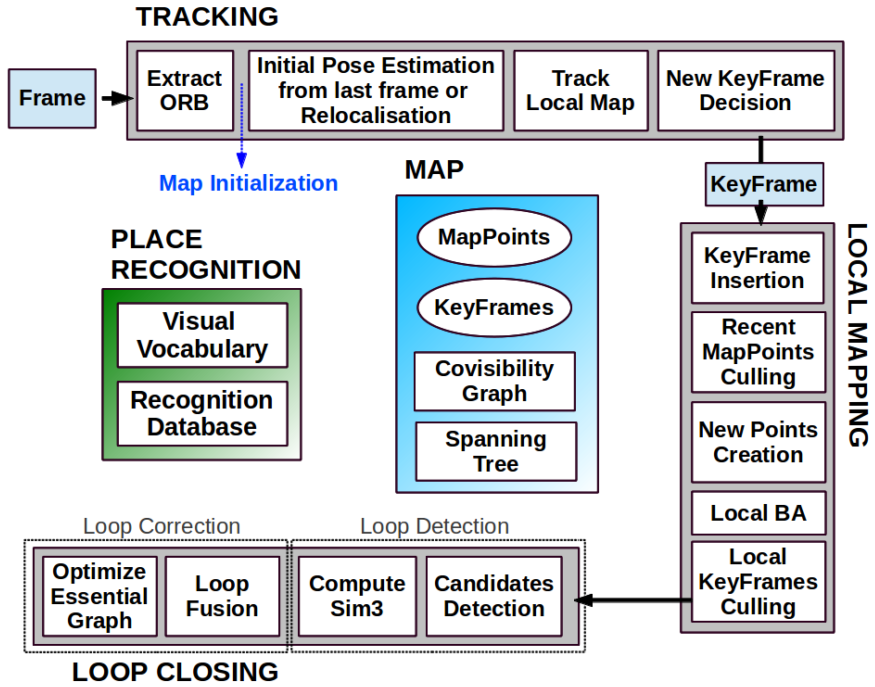
\includegraphics[width=0.6\textwidth]{figure/orb.png}
    \caption{ORB-SLAM主要分为三个线程进行,也就是如图所示的,分别是Tracking、LocalMapping和LoopClosing}
\end{figure}

\begin{enumerate}
        \item 跟踪(Tracking)\\ 这一部分主要工作是从图像中提取ORB特征,根据上一帧进行姿态估计,或者进行通过全局重定位初始化位姿,然后跟踪已经重建的局部地图,优化位姿,再根据一些规则确定新的关键帧。
        \item 建图(LocalMapping)\\ 这一部分主要完成局部地图构建。包括对关键帧的插入,验证最近生成的地图点并进行筛选,然后生成新的地图点,使用局部捆集调整(Local BA),最后再对插入的关键帧进行筛选,去除多余的关键帧。
        \begin{align}
                \{\mathbf{R}, \mathbf{t}\}=\underset{\mathbf{R}, \mathbf{t}}{\operatorname{argmin}} \sum_{i \in \mathcal{X}} \rho\left(\left\|\mathbf{x}_{(\cdot)}^{i}-\pi_{(\cdot)}\left(\mathbf{R} \mathbf{X}^{i}+\mathbf{t}\right)\right\|_{\Sigma}^{2}\right)
        \end{align}
        \item 闭环检测(LoopClosing)\\ 这一部分主要分为两个过程,分别是闭环探测和闭环校正。闭环检测先使用WOB进行探测,然后通过Sim3算法计算相似变换。闭环校正,主要是闭环融合和Essential Graph的图优化。
\end{enumerate}

\textbf{开源代码链接:}
\url{https://github.com/raulmur/ORB_SLAM2}

\subsubsection{多传感器融合:VINS-Mono}
该算法\cite{8421746}是一种鲁棒且通用的单目视觉惯性状态估计器。采用一种基于紧耦合、非线性优化的方法,通过融合预积分后的IMU测量值和特征观测值,获得高精度的视觉惯性里程计。结合紧耦合方法,回环检测模块能够以最小的计算代价实现重定位。
处理视觉和惯性测量的最简单的方法是松耦合的传感器融合\cite{8576618,8630025},其中IMU被视为一个独立的模块,用于辅助运动的视觉结构(sfm)获得的纯视觉位姿估计。融合通常由扩展卡尔曼滤波(EKF)完成,其中IMU用于状态传播,而视觉位姿用于更新。
  
\textbf{IMU预积分(pre-integration)}

在实践中,IMU通常以比摄像机更高的速率获取数据。不同的方法被提出来处理高速率的IMU测量值。最简单的方法是在基于EKF的方法中使用IMU进行状态传播[11][13]。在图优化公式中,为了避免重复的IMU重复积分,提出了一种有效的方法,即IMU预积分(IMU pre-integration)。
通过一系列计算,得到下面的预积分估计值:
\begin{align} 
\hat{\boldsymbol{\alpha }}^{b_k}_{i+1} &= \hat{\boldsymbol{\alpha }}^{b_k}_i + \hat{\boldsymbol{\beta }}^{b_k}_i\delta t + \frac{1}{2} \mathbf {R}(\hat{\boldsymbol{\gamma }}^{b_k}_i)(\hat{\mathbf {a}}_i - \mathbf {b}_{a_i}) \delta t^2 \nonumber\\ \hat{\boldsymbol{\beta }}^{b_k}_{i+1} &= \hat{\boldsymbol{\beta }}^{b_k}_{i} + \mathbf {R}(\hat{\boldsymbol{\gamma }}^{b_k}_i)(\hat{\mathbf {a}}_i - \mathbf {b}_{a_i})\delta t\nonumber\\ \hat{\boldsymbol{\gamma }}^{b_k}_{i+1} &= \hat{\boldsymbol{\gamma }}^{b_k}_i \otimes {\left[\begin{array}{c}1\\ \frac{1}{2} (\hat{\boldsymbol{\omega }}_i- \mathbf {b}_{w_i})\delta t \end{array}\right]}
\end{align}
通过计算可以写下IMU测量模型所其对应的协方差${\mathbf {P}^{b_k}_{b_{k+1}}}$:
\begin{equation} 
{\left[\begin{array}{c}\hat{\boldsymbol{\alpha }}^{b_k}_{b_{k+1}}\\ \hat{\boldsymbol{\beta }}^{b_k}_{b_{k+1}}\\ \hat{\boldsymbol{\gamma }}^{b_k}_{b_{k+1}}\\ \mathbf {0}\\ \mathbf {0}\\ \end{array}\right]} = {\left[\begin{array}{c}\mathbf {R}^{b_k}_{w}(\mathbf {p}^{w}_{b_{k+1}} - \mathbf {p}^{w}_{b_k} + \frac{1}{2}\mathbf {g}^{w} \Delta t_k^2 - \mathbf {v}^{w}_{b_k} \Delta t_k) \\ \mathbf {R}^{b_k}_{w}(\mathbf {v}^{w}_{b_{k+1}} + \mathbf {g}^{w} \Delta t_k- \mathbf {v}^{w}_{b_k}) \\ \mathbf {q}^{w^{-1}}_{b_{k}} \otimes \mathbf {q}^{w}_{b_{k+1}}\\ {\mathbf {b}_a}_{b_{k+1}} - {\mathbf {b}_a}_{b_k}\\ {\mathbf {b}_w}_{b_{k+1}} -{\mathbf {b}_w}_{b_k}\\ \end{array}\right]}.
\end{equation}

\textbf{估计器初始化}

单目紧耦合VIO是一个高度非线性的系统。由于单目相机无法直接观测到尺度,因此,如果没有良好的初始值,很难直接将这两种测量结果融合在一起。
当IMU测量结果被大偏置破坏时,情况就变得更加复杂了。事实上,初始化通常是单目VINS最脆弱的步骤。需要一个鲁棒的初始化过程以确保系统的适用性。
通过对齐IMU预积分与纯视觉SfM结果,我们可以粗略地恢复尺度、重力、速度,甚至偏置。这足以引导非线性单目VINS估计器。

\begin{figure}[H]
        \centering
        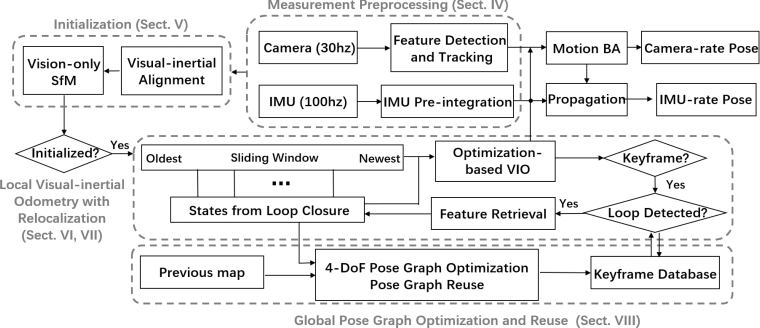
\includegraphics[width=0.6\textwidth]{figure/vins2.png}
        \caption{总体架构图}
\end{figure}

\textbf{开源代码链接:}
\url{https://github.com/HKUST-Aerial-Robotics/VINS-Mono}

\subsection{路径规划算法描述}

\subsubsection{总体概述}
路径规划是导航系统的一部分,其总结来看可以分为全局规划层(global planner)和局部规划层(local planner)。


\begin{figure}[h]
        \centering
        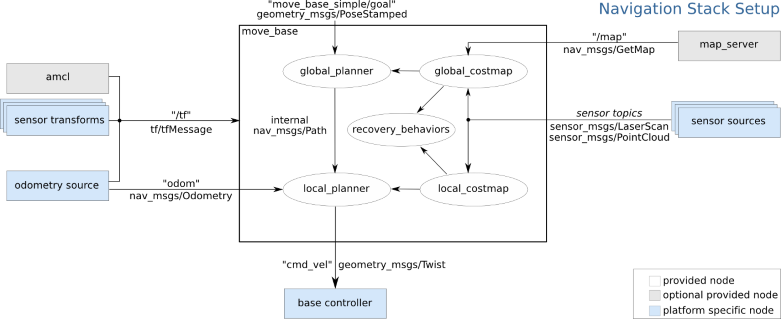
\includegraphics[width=0.8\textwidth]{figure/navigation.png}
        \caption{导航总体架构图}
\end{figure}

\subsubsection{代价地图的建立}
代价地图(COSTMAP)是一种机器人收集传感器信息建立和更新的二维或三维地图。
在ROS中,红色部分代表costmap中的障碍物,蓝色部分表示通过机器人内切圆半径膨胀出的障碍,红色多边形是footprint(机器人轮廓的垂直投影)。
红色部分代表costmap中的障碍物,蓝色部分表示通过机器人内切圆半径膨胀出的障碍,红色多边形是footprint(机器人轮廓的垂直投影)。可以从下图简要了解。
\begin{figure}[H]
        \centering
        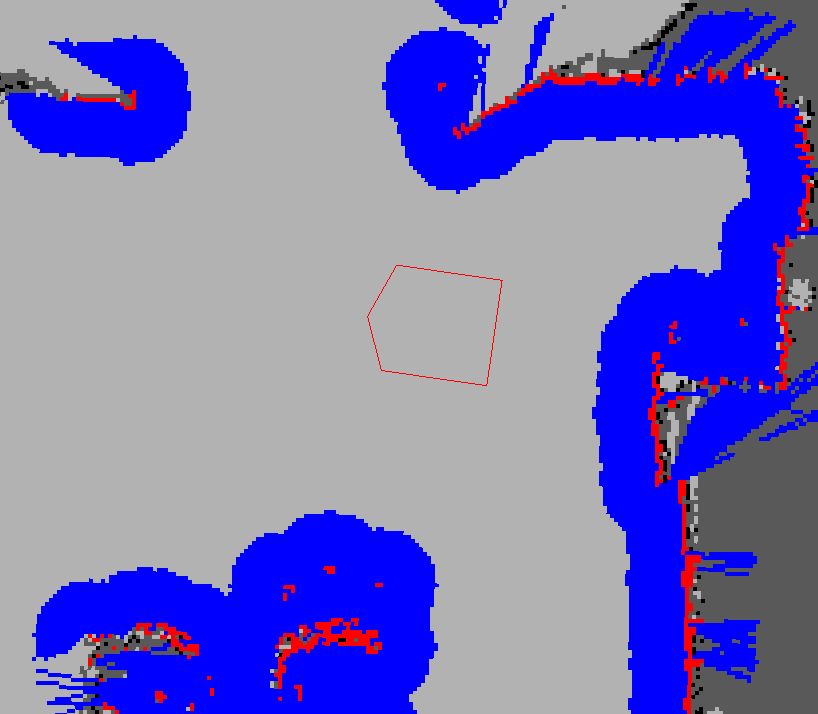
\includegraphics[width=0.5\textwidth]{figure/costmap.png}
        \caption{代价地图表示形式}
\end{figure}
ROS的代价地图(costmap)采用网格(grid)形式,每个网格的值(cell cost)从0~255。分成三种状态:被占用(有障碍)、自由区域(无障碍)、未知区域。
其原理也可以由下图得出。
\begin{figure}[H]
        \centering
        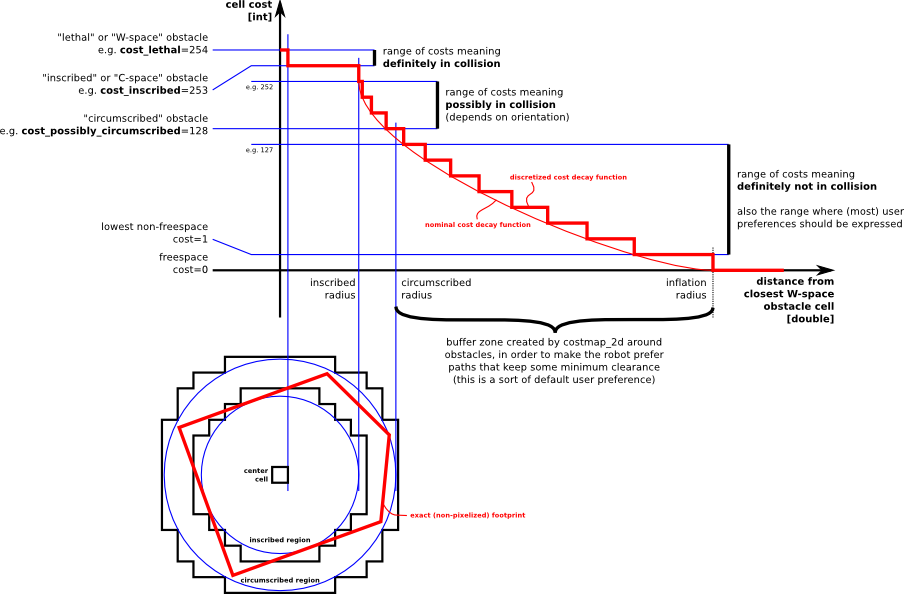
\includegraphics[width=0.7\textwidth]{figure/occupy.png}
        \caption{代价地图原理}
\end{figure}
\subsubsection{代价地图的更新}
通过不断地接受激光雷达扫描的数据(laserScan),不断更新代价地图(costmap)。由下图\cite{6942562}可以看到代价地图的生成流程。
\begin{figure}[H]
        \centering
        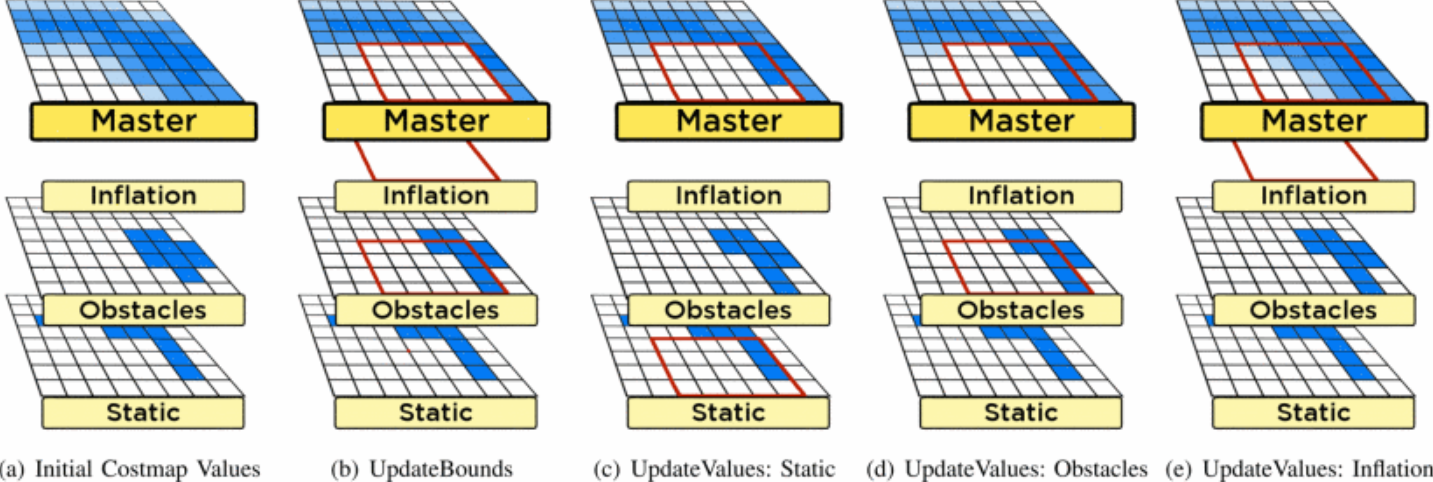
\includegraphics[width=0.7\textwidth]{figure/occupy1.png}
        \caption{代价地图生成过程}
\end{figure}

\subsubsection{全局路径规划:Dijskra}
该算法\cite{8784487}由经典最短路径算法Dijskra在2D占据地图上的应用得到。
是一种静态路网中求解最短路径最有效的直接搜索方法,也是解决许多搜索问题的有效算法。算法中的距离估算值与实际值越接近,最终搜索速度越快。 公式表示为:
\begin{align}
        f(n)=g(n)+h(n)
\end{align}
其中$f(n)$是从初始状态经由状态n到目标状态的代价估计,$g(n)$是在状态空间中从初始状态到状态n的实际代价,$h(n)$是从状态n到目标状态的最佳路径的估计代价。对于路径搜索问题,状态就是图中的节点,代价就是距离。

\subsubsection{全局路径规划:RRT*的改进方法}
该算法\cite{6942562}由RRT改进而来,同时对轨迹进行了平滑处理。该算法方法通常能用更小的树在更短的时间内产生更平滑的路径。对于 RRT*,该方法还生成最短路径,并在给定更多规划时间时实现成本最低的解决方案。

\textbf{1) RRT / RRT* 的特点}

通过抽样来在已知的地图上建立无向图,进而通过搜索方法寻找相对最优的路径。不同点在于,PRM算法在一开始就通过抽样在地图上构建出完整的无向图,再进行图搜索;而RRT算法则是从某个点出发一边搜索,一边抽样并建图。

\textbf{2) RRT / RRT* 的缺点}

RRT算法是概率完备的:只要路径存在,且规划的时间足够长,就一定能确保找到一条路径解。注意“且规划的时间足够长”这一前提条件,说明了如果规划器的参数设置不合理(如搜索次数限制太少、采样点过少等),就可能找不到解。

\textbf{3) 改进方法:POSQ}

由于RRT产生了很多点,所以根据原来的反馈方程,目标会在每个点处停下来。本方法通过修改反馈方程,使得在多次扩展中的恒定正向速度有所需的最大值。即以下闭环模型:
\begin{align}
        &\dot{\rho}=-K_{\rho}\cos\alpha\tanh(K_{v}\rho), \cr &\dot{\alpha}=K_{\rho}{\sin\alpha\over \rho}\tanh(K_{v}\rho)-K_{\alpha}\alpha-K_{\phi}\phi, \cr &\dot{\phi}=-K_{\alpha}\alpha-K_{\phi}\phi.
\end{align}
由此得到如图所示效果:
\begin{figure}[H]
        \centering
        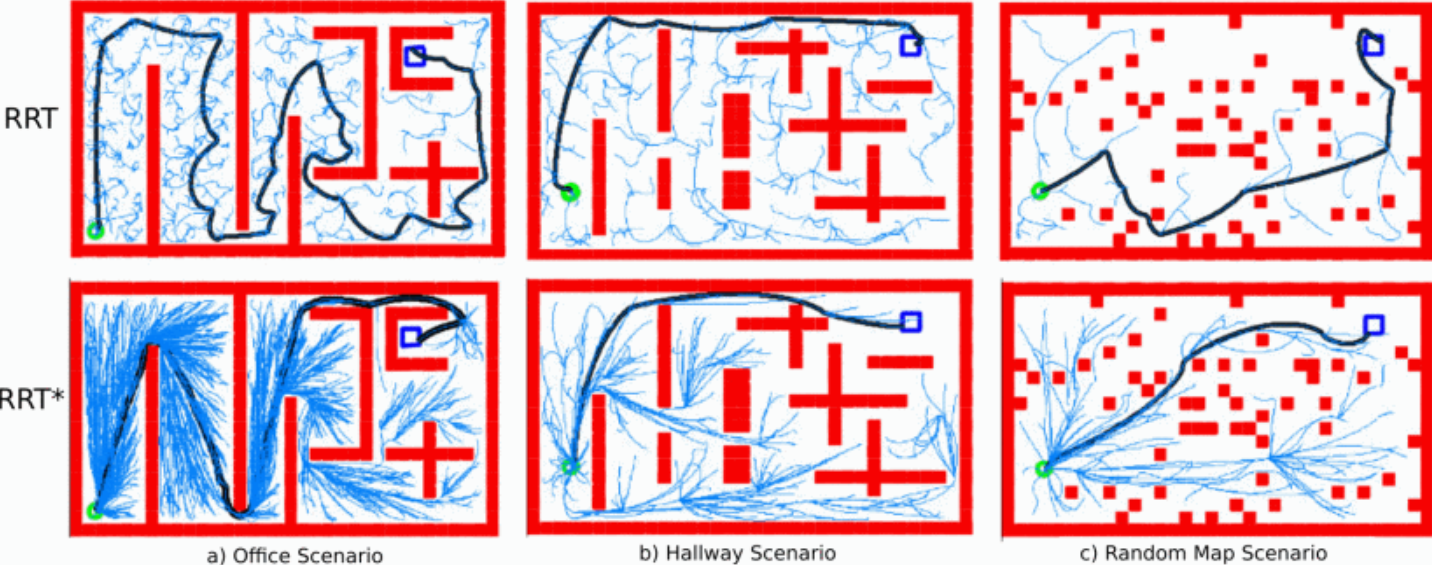
\includegraphics[width=0.7\textwidth]{figure/rrt-extend.png}
        \caption{RRT-EXTEND的效果图}
\end{figure}

\subsection{AGV姿态控制算法描述}
\subsubsection{AGV姿态控制}
随着工业物流技术的进步,AGV已越来越广泛地应用于工业制造和仓储场景。为了使AGV适应不同的工作场景,提高运行稳定度,AGV车身需及时响应计划的路径,完成物理位置及车身姿态的变换。控制方法为,在AGV车身的每一侧安装一个直流电动机,两个直流电动机安装有编码器,控制器通过编码器的反馈,控制电动轮的旋转,实现物理位置及车身姿态的变换。通过使用PID控制,AGV系统可以根据计划的路径快速改变位姿并修正错误。
\subsubsection{AGV的运动学分析}
2轮差速驱动AGV,即AGV的2驱动轮分别由1台直流伺服电机驱动。2驱动轮安装在车体的中间部位,车体前后各有1个万向轮支撑。AGV在绝对坐标系中可简化为图3.9所示模型\cite{杨远航基于模糊控制的}。图中L为AGV左右轮之间的距离,D为驱动轮直径,$\omega_{L}$、$\omega_{L}$、$\omega$ 分别为左轮、右轮和车体 转动角速度,$v_{L}$、$v_{R}$、$v$分别为左轮、右轮和车体几何 中心线速度。左、右轮的运动学方程分别为
\begin{align}
        \dot{x} \cos \theta+\dot{y} \sin \theta-\frac{L}{2} \dot{\theta}=\frac{D}{2} \omega_{\mathrm{L}}=v_{\mathrm{L}}\\ \dot{x} \cos \theta+\dot{y} \sin \theta-\frac{L}{2} \dot{\theta}=\frac{D}{2} \omega_{\mathrm{R}}=v_{\mathrm{R}}
\end{align}
\begin{figure}[H]
    \centering
    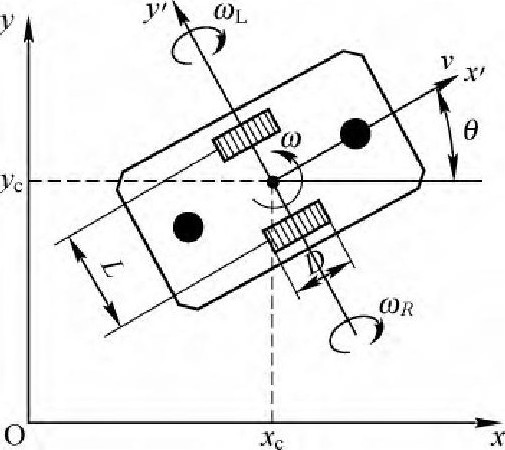
\includegraphics[width=0.7\textwidth]{figure/AGVkinematics.jpg}
    \caption{AGV运动学模型}
\end{figure}

AGV车体转动角速度
\begin{align}
    \omega=\dot{\theta}=\frac{\omega_{\mathrm{R}} r-\omega_{\mathrm{L}} r}{L}=\frac{v_{\mathrm{R}}-v_{\mathrm{L}}}{L}
\end{align}

AGV车体几何中心的线速度
\begin{align}
    v=\frac{\omega_{\mathrm{n}} r+\omega_{\mathrm{L}} r}{2}=\frac{v_{\mathrm{R}}+v_{\mathrm{L}}}{2}
\end{align}

式中:驱动轮的半径$r=\frac{D}{2}$。

定义速度向量
\begin{align}
    U=\left[\begin{array}{l}
        v \\
        \omega
        \end{array}\right]=\left[\begin{array}{cc}
        1 / 2 & 1 / 2 \\
        -1 / L & 1 / L
        \end{array}\right]\left[\begin{array}{l}
        v_{L} \\
        v_{R}
        \end{array}\right]
\end{align}

假设车轮与地面之间只有滚动,没有滑动,即满足理想约束情况,有
\begin{align}
    \dot{x} \cos \theta-\dot{y} \sin \theta = 0
\end{align}

则 AGV 的运动学方程可以表示为
\begin{align}
    \left[\begin{array}{c}
        \dot{x} \\
        \dot{y} \\
        \dot{\theta}
        \end{array}\right]=\left[\begin{array}{cc}
        \cos \theta & 0 \\
        \sin \theta & 0 \\
        0 & 1
        \end{array}\right]\left[\begin{array}{l}
        v \\
        \omega
        \end{array}\right]
\end{align}

由AGV的运动学方程可看出,通过控制AGV车体线速度v和角速度ω,即可实现AGV在绝对坐标系中不同位姿的运动。
\subsubsection{AGV姿态控制算法}
导航控制算法控制机器人沿着规划路径行驶。为了快速准确地跟踪目标点,PID作为主要的调节器\cite{8623691}。计算由摄像头与IMU及轮速计经卡尔曼滤波融合检测到的AGV行程轨迹的航向偏差和航向偏差作为PID控制器的输入,并将姿态调整量用作输出,控制器实现对预定路径的跟踪。PID控制原理图如图3.10所示。
\begin{figure}[H]
    \centering
    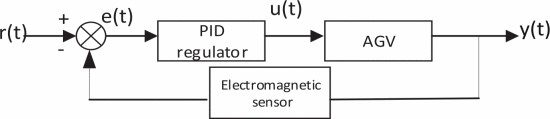
\includegraphics[width=0.7\textwidth]{figure/PIDcontroller.jpg}
    \caption{PID控制原理图}
\end{figure}
离散点的PID表达式为
\begin{align}
    u(k)=K_{p} \left\{e(k)+\frac{T}{T_{I}}\sum\limits_{i=0}^{k}e(i)+\frac{T_{d}}{T}[e(k)-e(k-1)\right\}
\end{align}

其中$K_{p}$是比例增益;$T_{I}$是积分系数,$T_{d}$是微分时间常数;$u(k)$是控制器采样为$k$时的输出;$T$是采样周期。

简化后
\begin{equation*}
    \Delta u(k)=K_{p}[e(k)-e(k-1)+K_{l}e(k)+K_{D}[e(k)-2e(k-1)+e(k-2)]
\end{equation*}

在公式中,比例增益决定系统的响应速度和控制精度,积分环节的作用是消除残差,提高控制性能,微分环节在大偏移发生前加快位姿修正的速率,从而快速完成小车轨迹的修正。因此,PID控制器可以有效地结合比例环节和微分环节的功能,既提高了系统的稳定性,又加快了系统的响应速度。

\subsection{基于RGBD的物体识别与定位算法描述}



\subsection{基于Web和MySQL的控制终端描述}
\subsubsection{机器人与服务器的通信}
为了实现上位机与多机器人间的通信,系统使用了基于TCP/IP协议簇的 Browser/ \\Server 模型,由于这种模型的客户端软件是 Web 浏览器,所以软件系统继 承了其跨平台的优点,不仅能通过电脑访问,也能通过其他任何带有浏览器功能的 移动设备访问。在TCP/IP模型中传输层的协议主要有两种传输控制协议,即面向连 接的TCP和面向无连接的用户数据报协议UDP。由于TCP中已经使用了大量数据 控制协议,能够保证数据传输的可靠性,因此本实验系统采用了面向连接的传输控 制协议TCP,它允许从一台机器发出的字节流能够无差错的发往到另一台机器。这样就不必重新构造一个保证可靠性的通信协议,缩短了软件开发的时间。

\subsubsection{网页与服务器通信}
由于网页前端是基于 http 协议的,一般只能通过请求和响应的形式来得到服务 器的信息,服务器也不能主动给网页前端发送消息,因此网页前端并不能通过Socket 技术与AGV的服务器通信,也就无法和小车通信了。因此在用户的网页前端与 Socket 客户端的通信方式上,常采用的是用户前端对服务端进行 Ajax 轮询。轮询 是在特定的时间间隔(如每 1 秒),用户的浏览器端对网页服务器发出 HTTP 请求, 然后由网页服务器返回最新的数据消息给用户端的浏览器,并保持这种通信模式直 到一方断开。这种传统的通信模式带来很明显的缺点,即浏览器需要不停的向服务 器发出请求,但是 HTTP 请求可能包含较长的头部,而其中真正有效的数据可能很 少,显然这样会浪费很多的系统资源。为了解决这一问题,可以使用HTML5中开 始提供的一种全新的全双规通讯协议WebSocket。WebSocket使得浏览器客户端和 网页服务器之间能快速的进行数据交换,允许服务端主动向客户端推送数据。由 WebSocket接收客户端的请求,并确定如何处理,即控制输入的请求和输出的回应。 用户控制界面使用WebSocket技术后,用户能通过WebSocket与AGV服务器进行 通信(图4.22),AGV服务器接收用户发送的控制命令后可以直接查询远端机器人 状态信息,并用相应的函数进行业务逻辑处理。
\section{实验部分}

\subsection{GUI控制程序演示}

\subsection{仿真模型构建}

\subsection{流程图}

\subsection{运行情况}

%===参考文献===
\addcontentsline{toc}{section}{参考文献}
\bibliographystyle{ieeetr}     %论文引用格式:缩写
\bibliography{conference_101719} %bib文件地址
\end{document}
%===结束===



